

\section{Comparison with other calibration methods {\color{LimeGreen} Laurence}}
\label{se:photometry_others}

The baseline calibration results are compared to
results drawn using other calibration methods that either resort to different
opacity correction or include a photometric correction to correct for
the beam impact. The 'taumeter' and 'skydip' methods are named from
the 'taumeter' and 'skydip' opacity corrections described in
Sect.~\ref{se:taumeter-method} and Sect.~\ref{se:skydip-method}
respectively. As the baseline calibration, these methods are based on
the baseline selection (see Sect.~\ref{se:data_selection}) for
discarding the scans that are the most impacted by the telescope-driven beam
effect. By contrast, 'photocorr demo' and 'photocorr pointing' use the
same opacity correction as the baseline method, that is 'corrected
skydip' (see Sect.~\ref{se:corrected-skydip}), but resort to the
'demo' and 'pointing' photometric corrections respectively, as
discussed in Sect.~\ref{se:photocorr_methods}. Using these
'photocorr' methods aleviate the need of a scan selection on the
observation date: all scans that meet the mild criteria based on
the atmospheric condition are included whatever the
observation date at which they have been acquired. 

\subsubsection{Calibration bias}

%%%%%%%%%%%%%%%%%%%%%%%%%%%%%%%%%%%%%%%%%%%%%%%%%%%%%%%%%%%%%%%%%%%%%%%%%%%%%%%%%%%%%%%%%%%%%
%                              bias
\begin{figure}[ht!]
  \begin{center}
    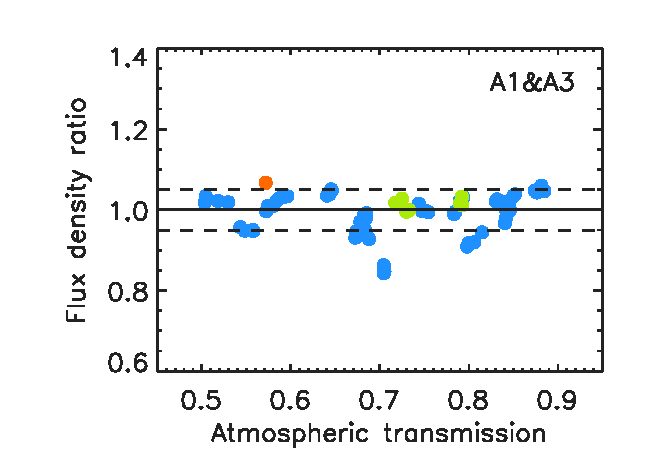
\includegraphics[clip=true, trim={0.9cm, 0.2cm, 0, 0.6cm},width=0.38\textwidth]{Figures/Calibration/plot_flux_density_ratio_MWC349_obstau_corrected_skydip_narrow_1mm.pdf}
    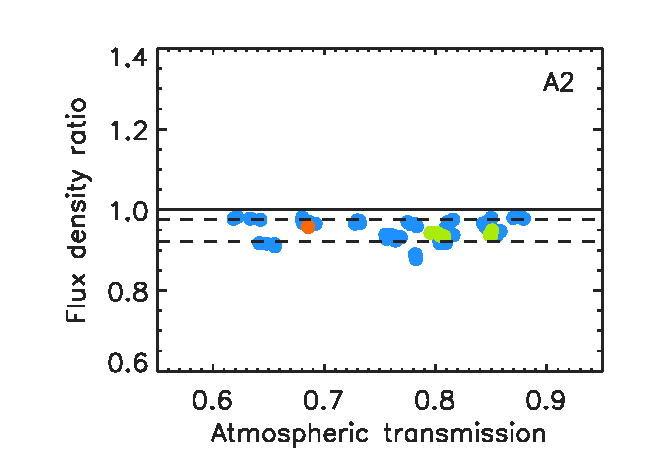
\includegraphics[clip=true, trim={0.9cm, 0.2cm, 0, 0.6cm},width=0.38\textwidth]{Figures/Calibration/plot_flux_density_ratio_MWC349_obstau_corrected_skydip_narrow_a2.pdf}
    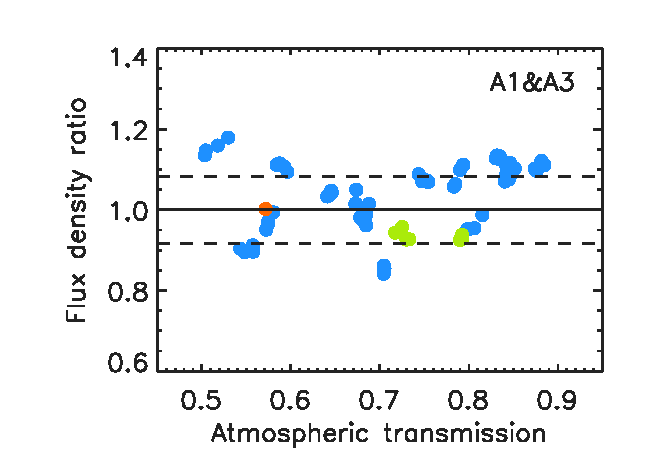
\includegraphics[clip=true, trim={0.9cm, 0.2cm, 0, 0.6cm},width=0.38\textwidth]{Figures/Calibration/plot_flux_density_ratio_MWC349_obstau_tau225_narrow_1mm.pdf}
    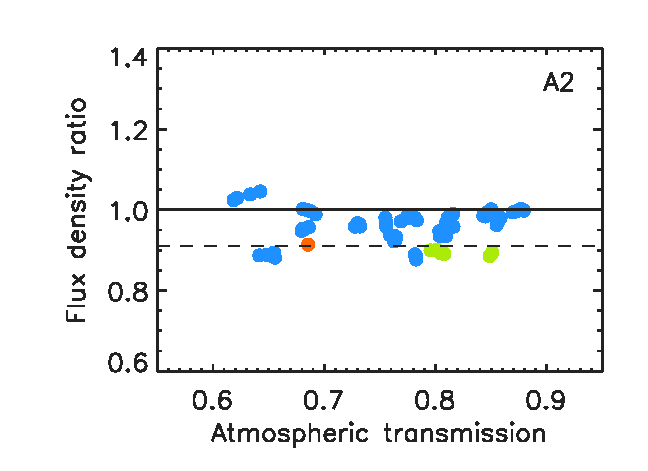
\includegraphics[clip=true, trim={0.9cm, 0.2cm, 0, 0.6cm},width=0.38\textwidth]{Figures/Calibration/plot_flux_density_ratio_MWC349_obstau_tau225_narrow_a2.pdf}
    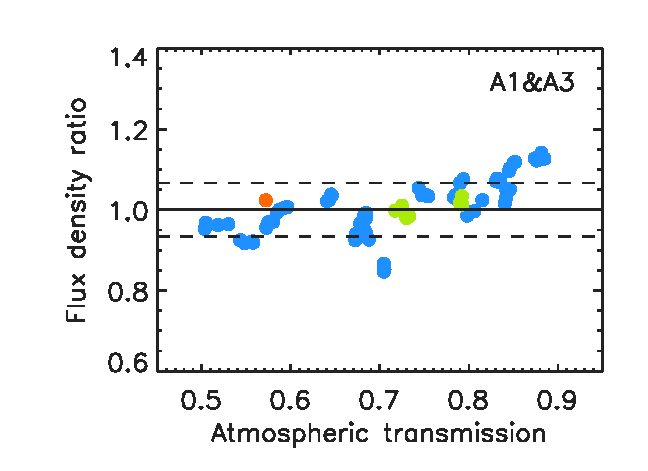
\includegraphics[clip=true, trim={0.9cm, 0.2cm, 0, 0.6cm},width=0.38\textwidth]{Figures/Calibration/plot_flux_density_ratio_MWC349_obstau_skydip_narrow_1mm.pdf}
    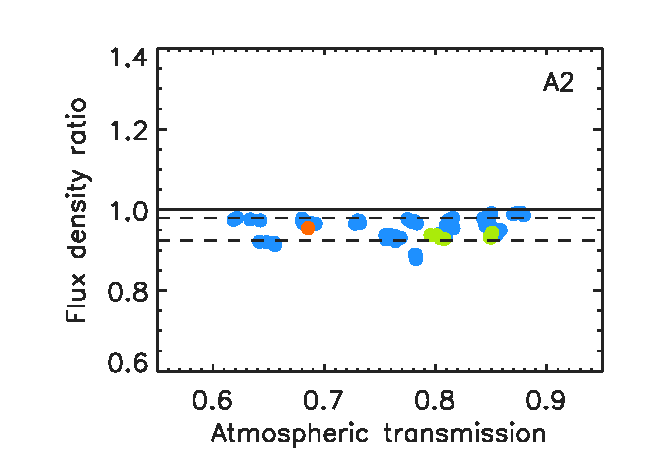
\includegraphics[clip=true, trim={0.9cm, 0.2cm, 0, 0.6cm},width=0.38\textwidth]{Figures/Calibration/plot_flux_density_ratio_MWC349_obstau_skydip_narrow_a2.pdf}
    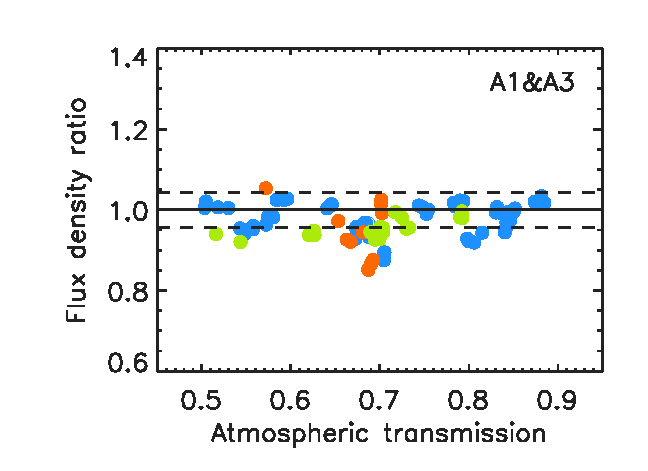
\includegraphics[clip=true, trim={0.9cm, 0.2cm, 0, 0.6cm},width=0.38\textwidth]{Figures/Calibration/plot_flux_density_ratio_MWC349_obstau_corrected_skydip_photocorr_demo_narrow_1mm.pdf}
    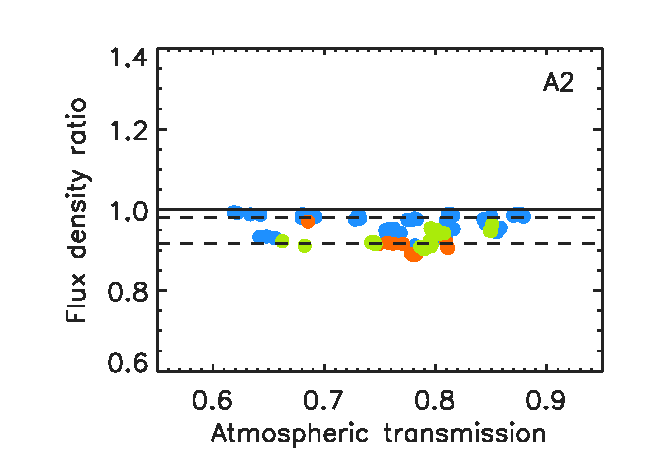
\includegraphics[clip=true, trim={0.9cm, 0.2cm, 0, 0.6cm},width=0.38\textwidth]{Figures/Calibration/plot_flux_density_ratio_MWC349_obstau_corrected_skydip_photocorr_demo_narrow_a2.pdf}
    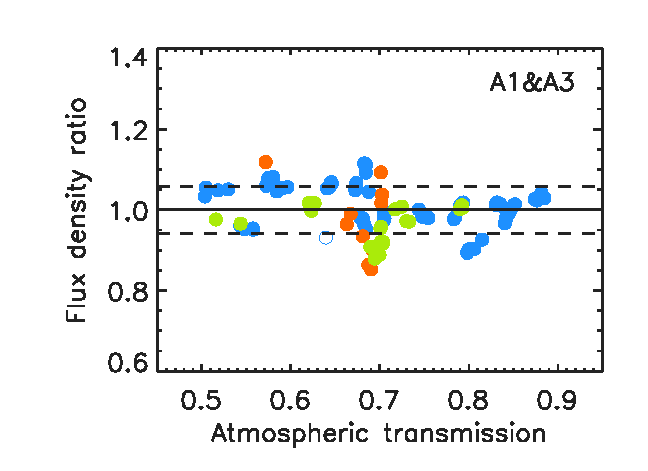
\includegraphics[clip=true, trim={0.9cm, 0.2cm, 0, 0.6cm},width=0.38\textwidth]{Figures/Calibration/plot_flux_density_ratio_MWC349_obstau_corrected_skydip_photocorr_pointing_narrow_1mm.pdf}
    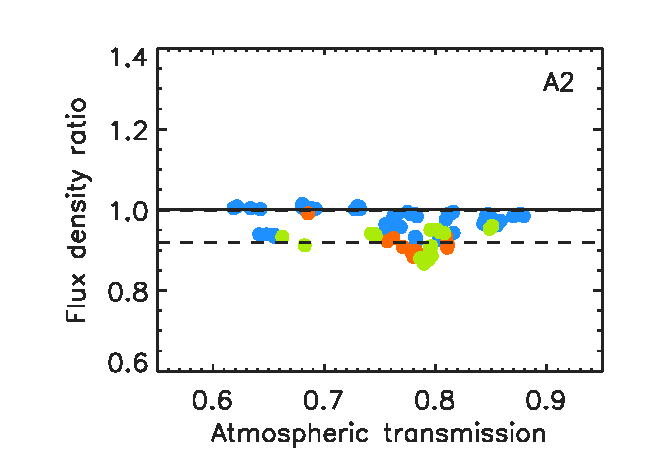
\includegraphics[clip=true, trim={0.9cm, 0.2cm, 0, 0.6cm},width=0.38\textwidth]{Figures/Calibration/plot_flux_density_ratio_MWC349_obstau_corrected_skydip_photocorr_pointing_narrow_a2.pdf}
    \caption[Calibration bias comparison]{Comparison of the
      calibration bias for five calibration methods. The measured-to-expected flux density ratio is shown as a
      function of the atmospheric transmission for the baseline method
      (first row) as well as for methods using the 'taumeter' (second
      row) and 'skydip' (third) opacity correction, and for methods
      resorting to the 'demo' (fourth) and 'pointing' (fifth)
      photometric correction. Dashed lines
      show the flux density ratio $1 \sigma $ dispersion.}
    \label{fig:mwc349_obstau_others}
  \end{center}
\end{figure}


% ALL METHOD RESULTS 
\begin{table}[th]
\begin{center}
\begin{tabular}{|c|l|c|c|c|c|c|}
  \hline
  \multicolumn{2}{|c|}{}  &  \multicolumn{5}{|c|}{Methods} \\\cline{3-7}
  \multicolumn{2}{|c|}{Characteristics} &  baseline  & taumeter  &  skydip  &  photocorr demo & photocorr pointing \\
  \hline\hline
  Bias &  $\#$ total    &   109   &   109    &   109    &    109    &  109   \\
       &  $\#$ selected &    72   &   72     &    72    &     96    &   95   \\
       &  A1            &   0.98  &  1.01    &  0.99    &   0.98    &  1.00  \\
       &  A3            &   1.00  &  1.04    &  1.01    &   1.01    &  1.02  \\
       &  1mm           &   1.00  &  1.03    &  1.00    &   1.00    &  1.01  \\
       &  2mm           &   0.95  &  0.96    &  0.95    &   0.95    &  0.95  \\
  \hline
  \multicolumn{7}{|l|}{Using color corrections as of Table A.1} \\
  \hline
  Bias &  A1            &   0.95   &  0.98    &  0.97    &   0.95    &  0.97  \\
       &  A3            &   1.00   &  1.02    &  1.02    &   0.99    &  1.00  \\
       &  1mm           &   0.98   &  1.01    &  1.00    &   0.97    &  0.99  \\
       &  2mm           &   0.95   &  0.95    &  0.95    &   0.95    &  0.95  \\
  \hline
  Rms  &  $\#$ total    &   487    &    487   &    487    &    396    &  396 \\
  $[\%]$     &  $\#$ selected &   264    &    264   &    264    &    291    &  283 \\
       &  A1            &   5.5    &    7.5   &    7.3    &    4.0    &  4.9 \\
       &  A3            &   6.0    &    8.1   &    7.1    &    4.1    &  5.2 \\
       &  1mm           &   5.7    &    7.9   &    7.1    &    3.8    &  4.9 \\
       &  2mm           &   3.0    &    3.8   &    3.0    &    2.2    &  2.4 \\
\hline\hline
\end{tabular}
\caption[Comparison of calibration results using five methods]{Comparison of calibration results using five methods}
\label{tab:Calibration_results_all}
\end{center}
\end{table}

We present the calibration bias (see the definition in
Sect.~\ref{se:photometry_criteria}) as a function of the atmospheric
transmission for the five calibration methods in
Fig.~\ref{fig:mwc349_obstau_others} and report the results in the row
labelled 'Bias' of Table~\ref{tab:Calibration_results_all}. 

At $1~\rm{mm}$, all methods lead to flux density estimates in
agreement with expectations within the rms dispersion. However,
'taumeter' ratios have more dispersion than the baseline method
ratios, whereas 'skydip' shows some dependency on the atmospheric
transmission, with a 10 to $15\%$ excess of the flux density with
respect to expectations at high transmission. These features, which are
already noticeable from Fig.~\ref{fig:mwc349_obstau_others}, will be
confirmed and further discussed using more scans. On an other hand,
the calibration methods based on photometric correction yield an
unbiased photometry (calibration bias in agreement with the unity
within the rms error) while using $30\%$ more scans. These results are
encouraging for the exploitation of scans acquired in difficult
observing condition. {\color{magenta} However, we note some difference between the
calibration bias using 'demo' and 'pointing', which indicates that
more extensive robustness tests are needed before routinely using the
practical method, \aka\ 'photocorr pointing'. NOT TRUE ANYMORE AFTER DEBUGGING}   


At $2~\rm{mm}$, all methods result in a similar calibration bias
of $0.95 \pm 0.05$. We also obtained the same $2\rm{mm}$-calibration
biases when using scans per campaign. To summarize, the
$2\rm{mm}$-calibration bias is stable against i) a large range of
atmospheric conditions, ii) the observation campaign, iii) the
opacity correction method, iv) the method to treat the beam
effect. An explanation for the $5\%$ lack of flux density toward
MWC349 is probably to be seeked on the side of the flux density
expectations for this source. Uncertainties on the
derivation of the flux density expectation comes in two flavours:
firstly, the accuracy of the SED fitted from PdB and VLA observations
depends on these instruments absolute calibration errors, which is
roughly estimated not to be better than $5\%$ for PdB, and secondly,
the NIKA2 flux density extrapolation from
interferometer data may be not straightforward for MWC349 (e.g. due to
the contamination by strong masers in the radio recombination lines~\cite{masingRRL}).
\addparag{more details on the sources of uncertainties on MWC349 flux
  expectations? Jean-Fran\c cois? }

\subsubsection{Calibration uncertainties}

%%%%%%%%%%%%%%%%%%%%%%%%%%%%%%%%%%%%%%%%%%%%%%%%%%%%%%%%%%%%%%%%%%%%%%%%%%%%%%%%%%%%%%%%%%%%%
%                              rms
\begin{figure}[ht!]
  \begin{center}
    % baseline
    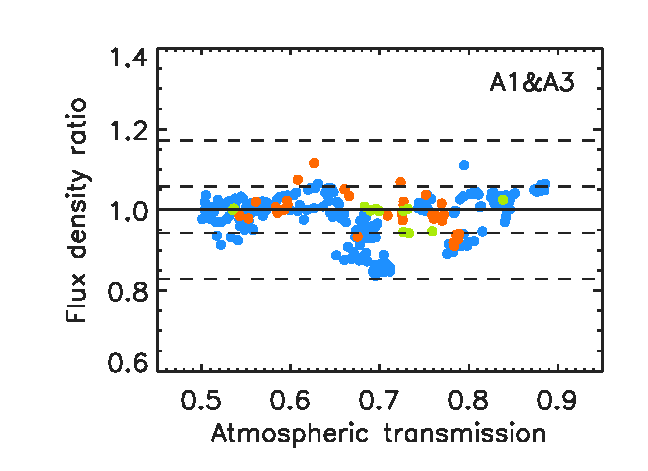
\includegraphics[clip=true, trim={0.9cm, 0.2cm, 0, 0.6cm}, width=0.32\textwidth]{Figures/Calibration/plot_flux_density_ratio_obstau_allbright_corrected_skydip_narrow_1mm.pdf}
    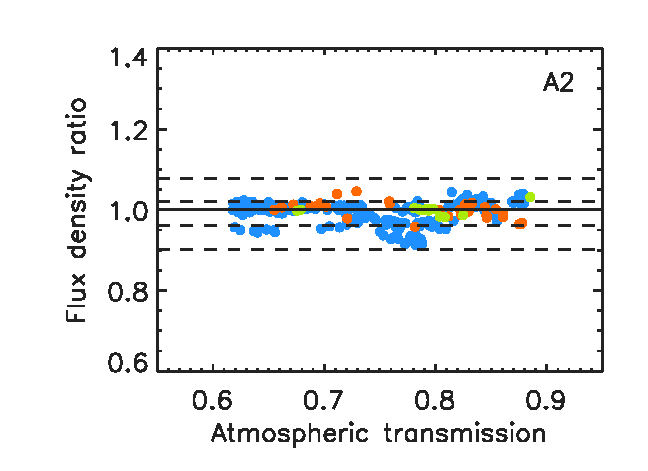
\includegraphics[clip=true, trim={0.9cm, 0.2cm, 0, 0.6cm}, width=0.32\textwidth]{Figures/Calibration/plot_flux_density_ratio_obstau_allbright_corrected_skydip_narrow_a2.pdf}
    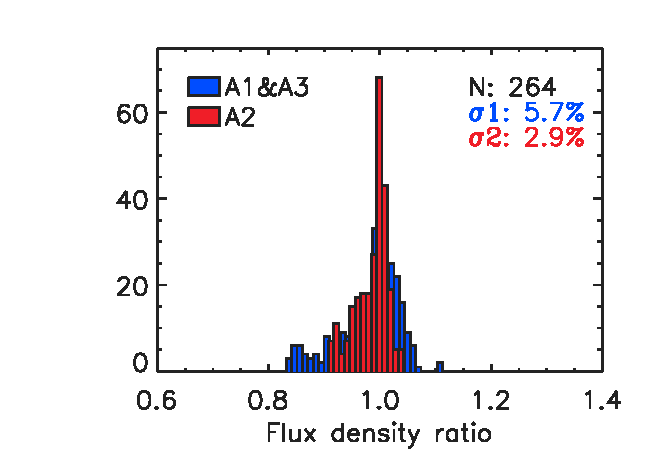
\includegraphics[clip=true, trim={0.9cm, 0.2cm, 0, 0.6cm}, width=0.32\textwidth]{Figures/Calibration/plot_histo_flux_density_ratio_obstau_allbright_corrected_skydip_narrow_1n2mm.pdf}
    % taumeter
    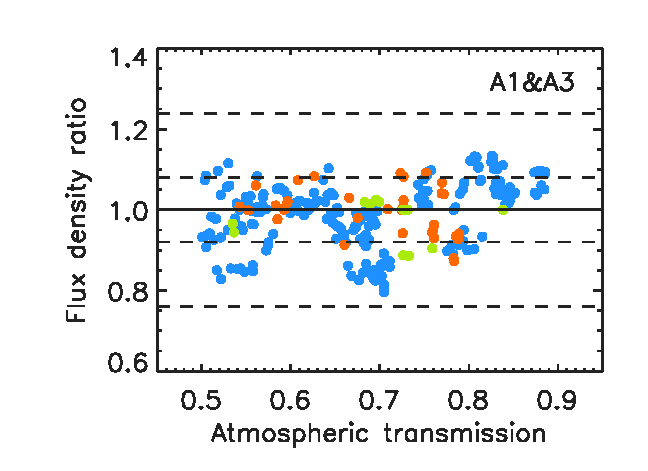
\includegraphics[clip=true, trim={0.9cm, 0.2cm, 0, 0.6cm}, width=0.32\textwidth]{Figures/Calibration/plot_flux_density_ratio_obstau_allbright_tau225_narrow_1mm.pdf}
    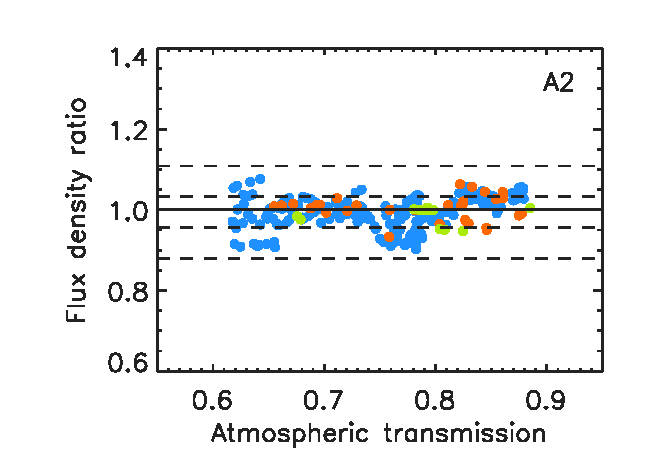
\includegraphics[clip=true, trim={0.9cm, 0.2cm, 0, 0.6cm}, width=0.32\textwidth]{Figures/Calibration/plot_flux_density_ratio_obstau_allbright_tau225_narrow_a2.pdf}
    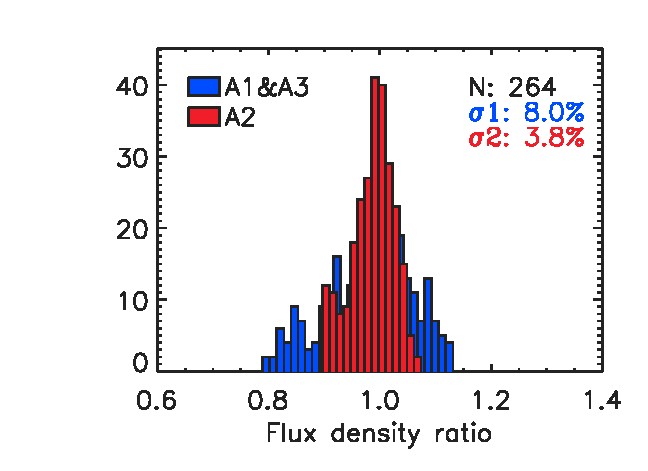
\includegraphics[clip=true, trim={0.9cm, 0.2cm, 0, 0.6cm}, width=0.32\textwidth]{Figures/Calibration/plot_histo_flux_density_ratio_obstau_allbright_tau225_narrow_1n2mm.pdf}
    % skydip
    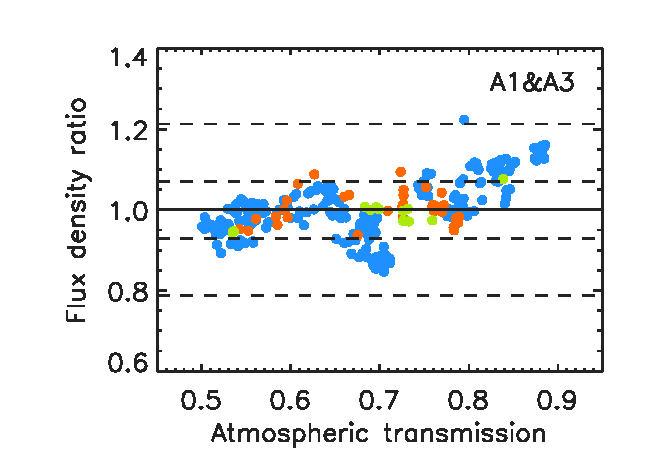
\includegraphics[clip=true, trim={0.9cm, 0.2cm, 0, 0.6cm}, width=0.32\textwidth]{Figures/Calibration/plot_flux_density_ratio_obstau_allbright_skydip_narrow_1mm.pdf}
    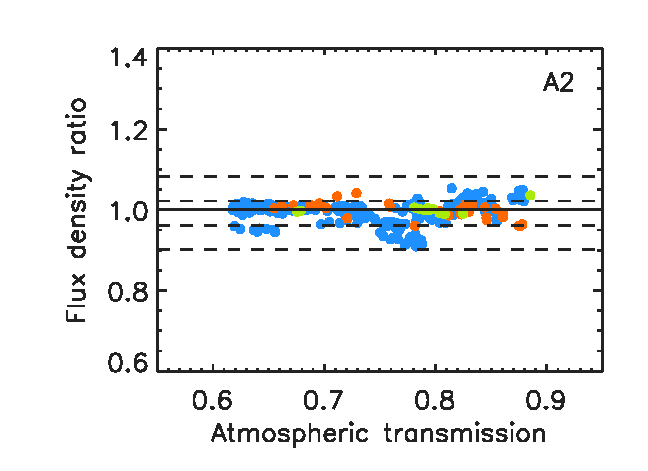
\includegraphics[clip=true, trim={0.9cm, 0.2cm, 0, 0.6cm}, width=0.32\textwidth]{Figures/Calibration/plot_flux_density_ratio_obstau_allbright_skydip_narrow_a2.pdf}
    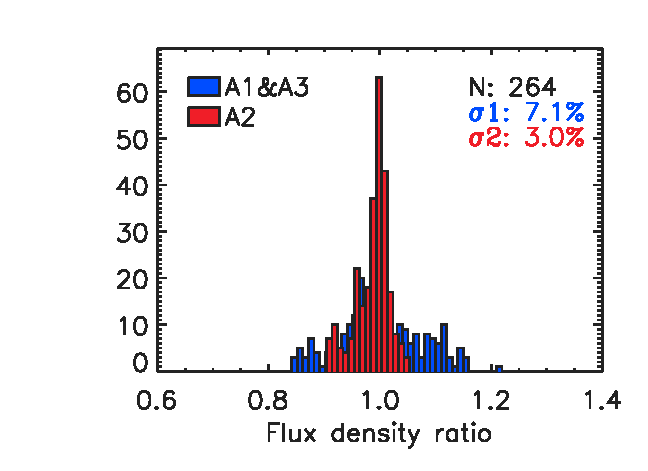
\includegraphics[clip=true, trim={0.9cm, 0.2cm, 0, 0.6cm}, width=0.32\textwidth]{Figures/Calibration/plot_histo_flux_density_ratio_obstau_allbright_skydip_narrow_1n2mm.pdf}
    % photocorr demo
    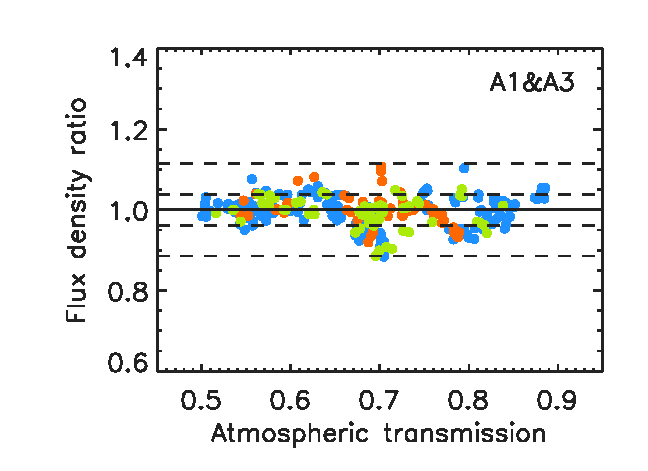
\includegraphics[clip=true, trim={0.9cm, 0.2cm, 0, 0.6cm}, width=0.32\textwidth]{Figures/Calibration/plot_flux_density_ratio_obstau_allbright_corrected_skydip_photocorr_demo_narrow_1mm.pdf}
    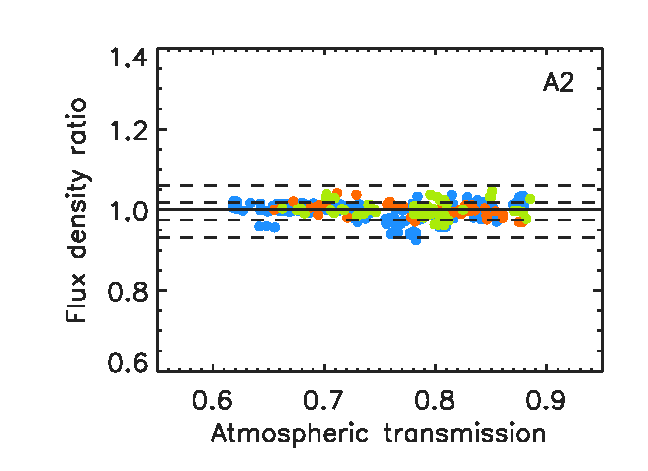
\includegraphics[clip=true, trim={0.9cm, 0.2cm, 0, 0.6cm}, width=0.32\textwidth]{Figures/Calibration/plot_flux_density_ratio_obstau_allbright_corrected_skydip_photocorr_demo_narrow_a2.pdf}
    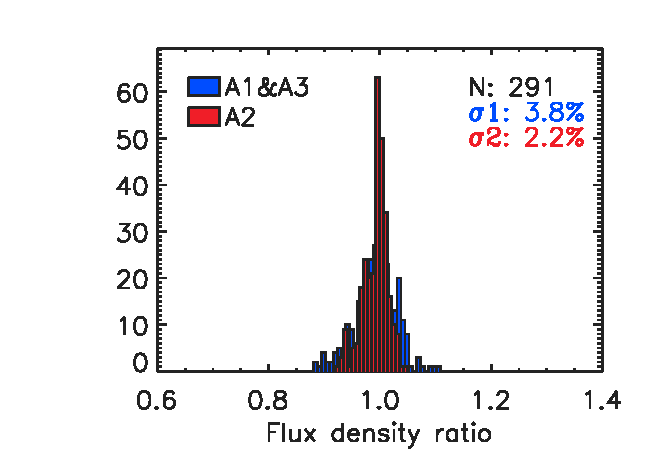
\includegraphics[clip=true, trim={0.9cm, 0.2cm, 0, 0.6cm}, width=0.32\textwidth]{Figures/Calibration/plot_histo_flux_density_ratio_obstau_allbright_corrected_skydip_photocorr_demo_narrow_1n2mm.pdf}
    % photocorr pointing
    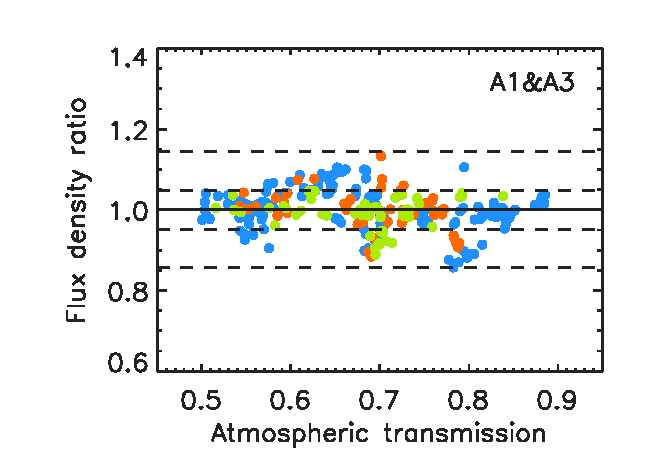
\includegraphics[clip=true, trim={0.9cm, 0.2cm, 0, 0.6cm}, width=0.32\textwidth]{Figures/Calibration/plot_flux_density_ratio_obstau_allbright_corrected_skydip_photocorr_pointing_narrow_1mm.pdf}
    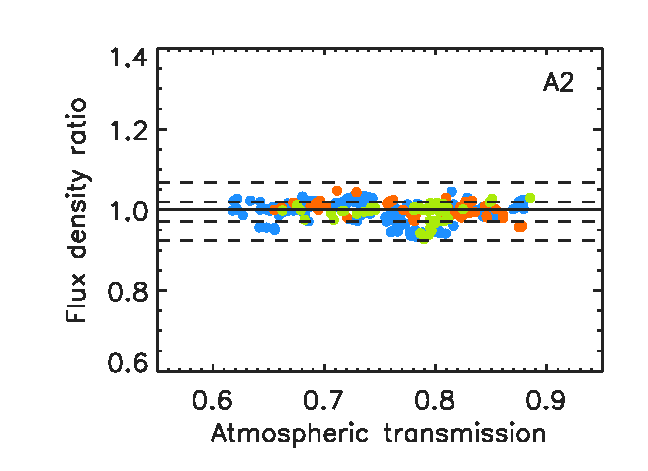
\includegraphics[clip=true, trim={0.9cm, 0.2cm, 0, 0.6cm}, width=0.32\textwidth]{Figures/Calibration/plot_flux_density_ratio_obstau_allbright_corrected_skydip_photocorr_pointing_narrow_a2.pdf}
    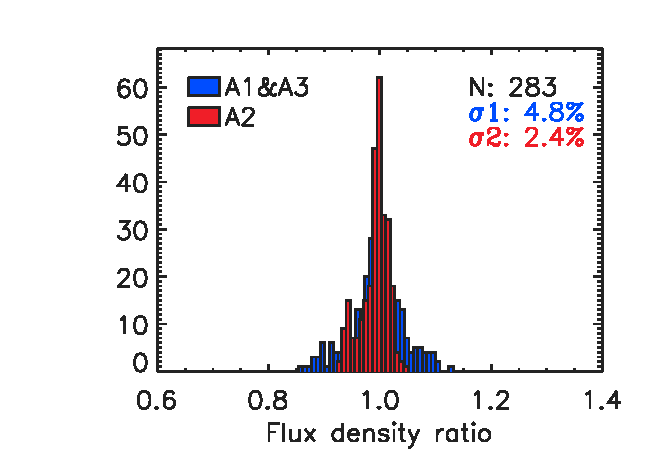
\includegraphics[clip=true, trim={0.9cm, 0.2cm, 0, 0.6cm}, width=0.32\textwidth]{Figures/Calibration/plot_histo_flux_density_ratio_obstau_allbright_corrected_skydip_photocorr_pointing_narrow_1n2mm.pdf}
    \caption[Comparison of calibration rms errors]{Comparison of the calibration uncertainties for five calibration methods. The
      measured-to-median flux density ratio at $1~\rm{mm}$ (first column) and $2~\rm{mm}$ (second column) of bright sources vs
      atmospheric transmission are shown as well as the flux density distibutions, using (first row) the baseline calibration, methods relying on (second row) the 'taumeter' and (third row) the 'skydip' opacity correction, and methods resorting to (fourth) row the 'demo' and (fifth row) the 'pointing' photometric correction.}
    \label{fig:allbright_rms_others}
  \end{center}
\end{figure}

We present the measured-to-median flux ratio versus the atmospheric
transmission at $1$ and $2~\rm{mm}$ and their distribution for the
five calibration methods in Fig.~\ref{fig:allbright_rms_others}, and
gather the derived calibration uncertainties in the row labelled 'Rms'
of Table~\ref{tab:Calibration_results_all}. From both these
information, we conclude that the 'taumeter' method leads to 
statistical uncertainty increases of about $40$ and $30\%$ at 1 and 2
mm. The 'skydip' method shows less dispersion but a correlation with
the atmospheric transmission. Although of a low significance (less
than $3\sigma$), this effect has motivated the development of the
'corrected skydip' method.

Comparing the flux density ratios using calibration methods with or
without photometry correction in Fig.~\ref{fig:allbright_rms_others},
we notice a clear difference for the bunch of N2R9 scans at an
atmospheric transmission of about 0.7: whereas the flux density ratios
are low for these scans in the three first methods, they are with
$1\sigma$ from unity when using a photometric correction. This further
validates the hypothesis that the low flux density of these scans is due to
telescope-driven beam effect, as assumed in
Sect.~\ref{se:photometry_baseline}. This also constitutes an example
of the calibration improvement obtained from resorting to a
photometric correction.

Moreover, results based on the 'photocorr demo' method show that calibration
uncertainties as low as $3.8$ and $2.2\%$
at 1 and 2 mm are within the reach of NIKA2 without rejecting any
observation dates. However, we recall this method relies on 
accurate beam estimates. Using the 'photocorr pointing', which is the
practical case, still decreases the calibration uncertainties
w.r.t. the baseline results but by a factor of about $20\%$ in both
bands. By inspecting the appropriate panels of
Fig.~\ref{fig:allbright_rms_others}, we notice some differences between
the flux density ratios from 'photocorr demo' and 'photocorr
pointing', which are likely to be due to the photometry correction noise
when monitoring the beam from pointing scans. We conclude that more
control on the beam monitoring is needed before proposing a calibration
based on photometry correction as the nominal method.


\subsubsection{Summary}

Amongst the methods that rely on the baseline scan selection to
mitigate the beam effect, the baseline method shows the best
performance in terms of calibration bias and uncertainties.

The lack of flux density at $2\sigma$ significance that was observed
for a small fraction of the N2R9 scans is confirmed to be due to the
telescope-driven beam effect.

Methods that rely on a photometric correction lead to good calibration
results: the calibration bias is in agreement with unity within
$1\sigma$ for the whole range of atmospheric transmissions and
calibration uncertainties as low as $3.8$ and $2.2\%$ have been obtained
without any scan selection based on the observation date. {\color{magenta}However,
evidence of a beam monitoring noise impact in the case of the
practical method (\aka\ 'photocorr pointing'), as well as difference
between results using the demonstration and the practical methods both
point to the need for further robustness tests before routinely use
these calibration methods. IS THAT STILL TRUE ?}
By contast, the baseline method allies good
performance and robustness.    








